\documentclass{article}
\usepackage{enumerate}
\usepackage{amsmath}
\usepackage{amssymb}
\usepackage{graphicx}
\usepackage{subfigure}
\usepackage{geometry}
\usepackage{caption}
\usepackage{indentfirst}
\geometry{left=3.0cm,right=3.0cm,top=3.0cm,bottom=4.0cm}
\renewcommand{\thesection}{Ex. \arabic{section} ---}
\title{VE475 Homework 1}
\author{Liu Yihao 515370910207}
\date{}

\begin{document}
\maketitle

\section{Simple questions}
\begin{enumerate}
\item
There are totally 26 possibilities of the plain text, which are listed below:

\begin{center}
\begin{tabular}{|c|c|c|c|}
\hline & $q_i$ & $r_i$ & $s_i$ \\\hline
0 & & 7467 & 1 \\\hline
1 & & 11413 & 0 \\\hline
2 & $ 7467\div11413=0$ & $7467-0\times11413=7467$ & $1-0\times0=1$ \\\hline
3 & $ 11413\div7467=1$ & $11413-1\times7467=3946$ & $0-1\times1=-1$ \\\hline
4 & $ 7467\div3946=1$ & $7467-1\times3946=3521$ & $1-1\times-1=2$ \\\hline
5 & $ 3946\div3521=1$ & $3946-1\times3521=425$ & $-1-1\times2=-3$ \\\hline
6 & $ 3521\div425=8$ & $3521-8\times425=121$ & $2-8\times-3=26$ \\\hline
7 & $ 425\div121=3$ & $425-3\times121=62$ & $-3-3\times26=-81$ \\\hline
8 & $ 121\div62=1$ & $121-1\times62=59$ & $26-1\times-81=107$ \\\hline
9 & $ 62\div59=1$ & $62-1\times59=3$ & $-81-1\times107=-188$ \\\hline
10 & $ 59\div3=19$ & $59-19\times3=2$ & $107-19\times-188=3679$ \\\hline
11 & $ 3\div2=1$ & $3-1\times2=1$ & $-188-1\times3679=-3867$ \\\hline
\end{tabular}
\end{center}


According to observation, RIVER and ARENA may be the secret place.

\item
Since the length of the text is 4, $n$ maybe 2, then we can construct an equation according to the plaintext \emph{dont} and the ciphertext \emph{ELNI}.
$$
\begin{pmatrix}3&14\\13&19\end{pmatrix}
\begin{pmatrix}a&b\\c&d\end{pmatrix}
\equiv\begin{pmatrix}4&11\\13&8\end{pmatrix}
{\rm\ mod\ }26
$$
$$
K=\begin{pmatrix}a&b\\c&d\end{pmatrix}\equiv
\begin{pmatrix}3&14\\13&19\end{pmatrix}^{-1}
\begin{pmatrix}4&11\\13&8\end{pmatrix}
{\rm\ mod\ }26
$$
$$
K=\begin{pmatrix}a&b\\c&d\end{pmatrix}\equiv
\begin{pmatrix}3&14\\13&19\end{pmatrix}^{-1}
\begin{pmatrix}4&11\\13&8\end{pmatrix}
{\rm\ mod\ }26
$$
$$\det\begin{pmatrix}3&14\\13&19\end{pmatrix}=-125$$
$$(-125)\cdot(-5)\equiv 1{\rm\ mod\ }26$$
$$
K=\begin{pmatrix}a&b\\c&d\end{pmatrix}\equiv
\begin{pmatrix}-95&70\\65&-15\end{pmatrix}
\begin{pmatrix}4&11\\13&8\end{pmatrix}
{\rm\ mod\ }26
$$
$$
K=\begin{pmatrix}a&b\\c&d\end{pmatrix}\equiv
\begin{pmatrix}9&18\\13&11\end{pmatrix}
\begin{pmatrix}4&11\\13&8\end{pmatrix}
{\rm\ mod\ }26
$$
$$
K=\begin{pmatrix}a&b\\c&d\end{pmatrix}\equiv
\begin{pmatrix}270&243\\195&231\end{pmatrix}
{\rm\ mod\ }26
$$
$$
K=\begin{pmatrix}10&9\\13&23\end{pmatrix}
$$

\item
Suppose that $n\nmid b$, let $b=cn+d$, $n\nmid d$ and $ab=kn$, where $c,d,k\in N$, then
$$a(cn+d)=kn$$
$$ad=(k-ac)n=\frac{ad}{n}n$$

We know $k-ac$ is an integer, so $\dfrac{ad}{n}$ is also an integer. However, since $\gcd(a,n)=1\Rightarrow n\nmid a$ and $n\nmid d$, it makes a contradiction, so $n\mid b$.

\item
\begin{align*}
30030&=116\times257+218\\
257&=1\times218+39\\
218&=5\times39+23\\
39&=1\times23+16\\
23&=1\times16+7\\
16&=2\times7+2\\
7&=3\times2+1\\
2&=2\times1
\end{align*}
$$\gcd(30030,257)=1$$

Since $16<\sqrt{257}<17$, so the factors of 257 can only be 2, 3, 5, 7, 11, 13, we can try them one by one. 257 mod 2 = 1, 257 mod 3 = 2, 257 mod 5 = 2, 257 mod 7 = 5, 257 mod 11 = 4, 257 mod 13 = 10. Then we can concluded that 257 is prime.

\item
If the attacker got the pair of a plaintext and its corresponding ciphertext of length $l$, he can just XOR the plaintext and the ciphertext to get the key of length $l$. When another message ciphered with the same key was sent, the attacker can easily decipher the ciphertext and steal the message. So using the same key twive in the OTP is dangerous.

\item
Since secure means that the attacker has to compute at least $2^{128}$ operations to break the encrypton, $$\sqrt{n\log n}\geqslant 128$$
$$n\geqslant4486.43$$

So  a graph with a size of 4487 should be used to be secure.

\end{enumerate}

\section{Vigenère cipher}
\begin{enumerate}
\item
Suppose we have a plaintext of length $l$ and a key of length $n$. First, if $n<l$, we repeat it for several times until it reach a length of $l$. Then, for each letter in the plaintext, we shift it by the value of the key letter of the same index as the letter, using the method similar to Caesar cipher.

For convenience, we obtain a Vigenère square, or Vigenère table, shown in Figure \ref{vigenere}. We can find the encrypted letter at the cross of the plaintext letter and the corresponding key letter.

When we want to decrypt the ciphertext, we can choose the row of the corresponding key letter and find the position of the letter in the ciphertext, then the letter of that column is the plaintext letter in that place.

\begin{figure}[t]
\centering
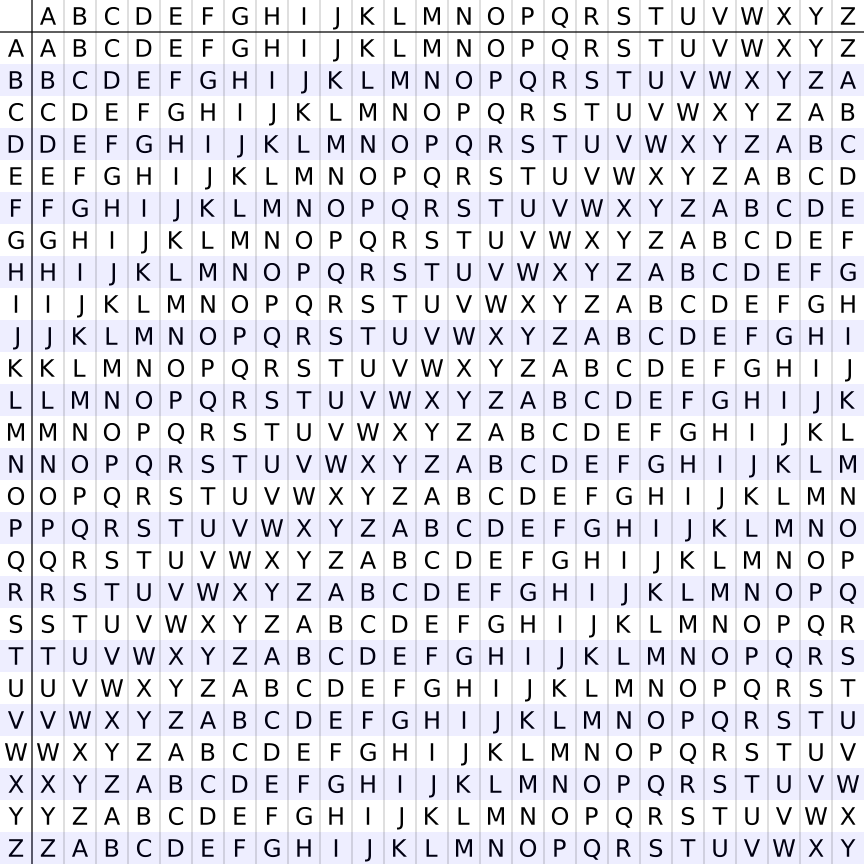
\includegraphics[scale=0.4]{vigenere.png}
\caption{Vigenère square}
\label{vigenere}
\end{figure}


\item
\begin{enumerate}[a)]
\item
If the plaintext is a same letter repeating hundreds of times, and the key have a length of $l$, then the ciphertext will have a loop every $l$ letters, it will be very obvious to observe in this circumstance. So Eve can suspect it.
\item
Eve can count the letters in each loop and easily find $l=6$.
\item
Eve can choose each of 26 letters one by one and compare with the first six letters of the ciphertext. According to the Vigenère square, he can get 26 possible keys with six letters. Since no English word of length six is a shift of another English word, only one of the 26 keys is the correct key, Eve can determine it with the help of an English dictionary.
\end{enumerate}
\end{enumerate}


\section{Programming}
Uploaded to Canvas.

\end{document}
